\chapter{Introducción}

Los bots son software que, mediante la ejecución de algoritmos, permiten automatizar tareas repetitivas de manera autónoma en un sistema. En los últimos años se ha popularizado mucho su uso, tanto es así que es raro no encontrarlos integrados en cualquier aplicación, ya sea de mensajería instantánea o de otros ámbitos. Dado su creciente popularidad, así como la de las plataformas sociales en las que se encuentran, cada día hay más usuarios que quieren hacer uso de ellos, ya sea en el ámbito laboral o simplemente a modo de ocio.

La plataforma \textit{Discord}, una aplicación de mensajería instantánea de texto y voz, es uno de los mejores ejemplos de la integración de bots en una plataforma social. En ella esta característica tiene gran aceptación y uso por parte de los usuarios. Esto, junto con la versatilidad de la aplicación, ha hecho que en los últimos años gane mucha popularidad\cite{tsbb}. 

Además, en contraste con otros sistemas de mensajería instantánea que también incorporan bots, como por ejemplo \textit{Telegram} o \textit{Slack}, es una de las aplicaciones donde el ritmo de crecimiento del uso de bots es más acusado\cite{enlyft}. Es por ello que cada vez más usuarios demandan la existencia de más bots y de que estos tengan más funcionalidades.

Sin embargo, aunque dado su intuitivo funcionamiento puedan parecer sencillos, todo lo que rodea a un bot puede llegar a ser intrincado. Este es el caso de su proceso de creación. Generalmente la creación de un bot requiere de una serie de procedimientos y conocimientos informáticos de la que no todos los usuarios disponen, así como de la implementación de una compleja infraestructura. Es por ello que actualmente su desarrollo está bastante limitado a usuarios con un nivel avanzado de conocimientos informáticos.

Existen algunas soluciones a este problema, que, en la medida de lo posible, intentan acercar la creación de bots a todo tipo de usuarios. Sin embargo, las herramientas que existen actualmente tienen bastantes limitaciones. En primer lugar, no se permite la creación de bots y comandos polivalentes, reduciéndose las posibilidades a unas pocas funcionalidades muy simples y predefinidas sin posibilidad de cambio. Además todas las herramientas existentes se basan en planes de pago, ofreciendo soluciones donde el usuario apenas tiene control de las funcionalidades de los bots.

El caso de la plataforma \textit{Discord} no es una excepción y tanto la creación como el despliegue de bots son procesos complejos. Es por ello que la simplificación del proceso de creación de estos ayudaría a que pudieran llegar a un mayor número de usuarios. Esta simplificación, a pesar de ser una tarea compleja, no es imposible.

Una solución adecuada debería incluir en primer lugar la unificación de todas las herramientas necesarias en cada una de las etapas del proceso de creación. Además, se debería crear un sistema que las facilite, sirviendo a modo de capa de abstracción. De gran importancia también sería que el problema se resuelva para los dos tipos de usuarios de \textit{Discord}, en concreto:

\begin{itemize}
	\item Usuarios que no tienen un conocimiento informático avanzado pero que buscan una herramienta versátil con la que crear bots y comandos de \textit{Discord} fácilmente y sin limitaciones.
	\item Usuarios con conocimiento informático avanzado que buscan una herramienta con la que crear bots y comandos de Discord sin limitaciones y, además, evitar tener que preocuparse de toda la infraestructura necesaria para crear y desplegar los bots.
\end{itemize}

Por otro lado, y en contraste con las soluciones actuales, sería ideal desarrollar una solución de software libre que cualquier usuario pueda utilizar y adaptar a sus necesidades. Dado su carácter gratuito, para poder obtener beneficio del software se podría implementar un modelo de consultoría, donde se desarrollen tanto soluciones personalizadas como se ofrezca el \textit{hosting} del sistema. Esto último sería de especial interés para aquellos usuarios con un menor conocimiento técnico.



\section{Motivación}

La principal motivación para realizar este proyecto es la ausencia de una herramienta de software libre que permita crear bots de \textit{Discord} de forma más simple tanto para usuarios con conocimientos con conocimientos técnicos avanzados, como para usuarios no expertos.

Crear una herramienta que facilite estos procesos podría:

\begin{itemize}
	\item Favorecer la comunidad de desarrollo de bots y de herramientas de creación de bots, permitiendo que los usuarios se centren en el desarrollo de las funcionalidades concretas en lugar de dedicar tiempo a otras tareas costosas y complejas de implementación de la infraestructura necesaria.
	\item Facilitar el acercamiento de los usuarios con menor conocimiento técnico a la creación y despliegue de bots.
	\item Favorecer la creación de software libre en este campo, que actualmente solo dispone de software propietario.
\end{itemize}

Aunque este problema suele ser general para todas las plataformas que permiten la integración de bots, este proyecto se centra el desarrollo para la plataforma \textit{Discord}. Esta elección se debe a que es la que probablemente podría beneficiarse más de un software de este tipo, dada la gran cantidad de usuarios que hace uso de ella y el éxito que está teniendo en multitud de ámbitos. Además, la  comunidad de desarrollo de bots para \textit{Discord} se encuentra en un momento de gran crecimiento y crear una herramienta que facilite los aspectos mencionados puede ser de gran utilidad.

Otro de los aspectos motivantes es el crear un software ampliable, es decir, que no se quede estancado una vez termine su desarrollo y que pueda extenderse de forma sencilla según las necesidades de los usuarios y/o novedades en el sector.



\section{Objetivos}

Este proyecto tiene los siguientes objetivos:

\begin{enumerate}
	\item Simplificar la creación de bots de \textit{Discord}, de modo que estos sean fácilmente extensibles y configurables frente al uso de recursos tradicionales de programación.
	\item Agilizar el proceso de despliegue de estos bots, de manera que se eliminen las trabas y procedimientos asociados al despliegue de estos sistemas.
	\item Facilitar la creación de comandos de \textit{Discord} de modo que estos sean sencillos de configurar, reutilizar y ampliar haciendo uso de herramientas de programación.
	\item Publicar versiones del software en los repositorios de imágenes de \textit{Docker} para facilitar la distribución del mismo.
	\item Reducir el tiempo de creación y despliegue de un bot de \textit{Discord} al menos en un 50\% frente al uso de herramientas de programación que permiten crear bots de este tipo.
\end{enumerate}



\section{Conceptos básicos}

En la siguiente sección se introducen todos aquellos conceptos y términos que se usan a lo largo de este documento y que es útil conocer y comprender para la lectura.



\subsection{Sistemas de mensajería instantánea}

Todos aquellos sistemas que permiten una comunicación basada en texto a través de la red en tiempo real entre usuarios. Además de mensajes, multitud de ellos permiten la comunicación a través de llamadas de voz o vídeo, envío de mensajes de audio, así como compartir documentos.

En general estos sistemas organizan la comunicación entre usuarios de distintas maneras, entre ellas las siguientes:

\begin{itemize}
	\item Conversaciones privadas. Chat privado entre dos usuarios.
	\item Grupos. Pequeñas comunidades de usuarios que permiten el intercambio de mensajes entre todos ellos.
	\item Canales. Análogo al grupo pero con la particularidad de que sólo el propietario del canal puede enviar mensajes a los usuarios suscritos.
\end{itemize}

Los protocolos que soportan estos sistemas son varios, y cada aplicación utiliza los que mejor se adecúan a las necesidades concretas. Algunos ejemplos son \textit{WebRTC}, \textit{WebSocket}, \textit{IRC} o \textit{XMPP}.

En lo que se refiere a la integración de bots en estos sistemas, es bastante usual, ya que aportan gran funcionalidad extra a estas aplicaciones. Generalmente los bots se ejecutan a nivel de sistema operativo, como un software más, por lo que no se ejecutan en los dispositivos de los usuarios, sino en servidores y/o máquinas remotas encargadas de alojar software de ese tipo. Aún así existen excepciones, y es posible ejecutar bots como plugins o extensiones de un software.



\subsection{\textit{Discord}}

Es una aplicación de mensajería instantánea multiplataforma semejante a otras herramientas que se usan en ámbitos similares, como \textit{Slack} o \textit{TeamSpeak}, y que ofrece distintos servicios de comunicación, como mensajería instantánea, chat de voz y vídeo e integración con bots y videojuegos, haciendo uso del protocolo \textit{WebRTC}.

La integración con bots en el caso de esta plataforma ha sido de gran importancia, ya que ha permitido que \textit{Discord} gane una gran visibilidad en los últimos años y se haya hecho muy popular, incluso en el ámbito profesional. La herramienta destaca frente a sus competidoras también en otros aspectos\cite{earthweb}, como la sencilla integración con otras herramientas (como videojuegos o \textit{Spotify}). Es por ello que en los últimos meses ha alcanzado más de 150 millones de usuarios activos al mes, siendo una de las aplicaciones más utilizadas hoy en día.

La principal forma de interacción de los usuarios en \textit{Discord} es a través de los llamados \textbf{servidores}. Estos son  comunidades de usuarios con un interés en común, ya sea en el ámbito personal (deportes, cine, etc) o profesional (equipos de trabajo). En cada servidor existen dos tipos de canales de comunicación: de texto, donde los usuarios pueden mandar mensajes; y de voz, donde los usuarios pueden conversar en tiempo real.

\begin{figure}[H]
	\centering
	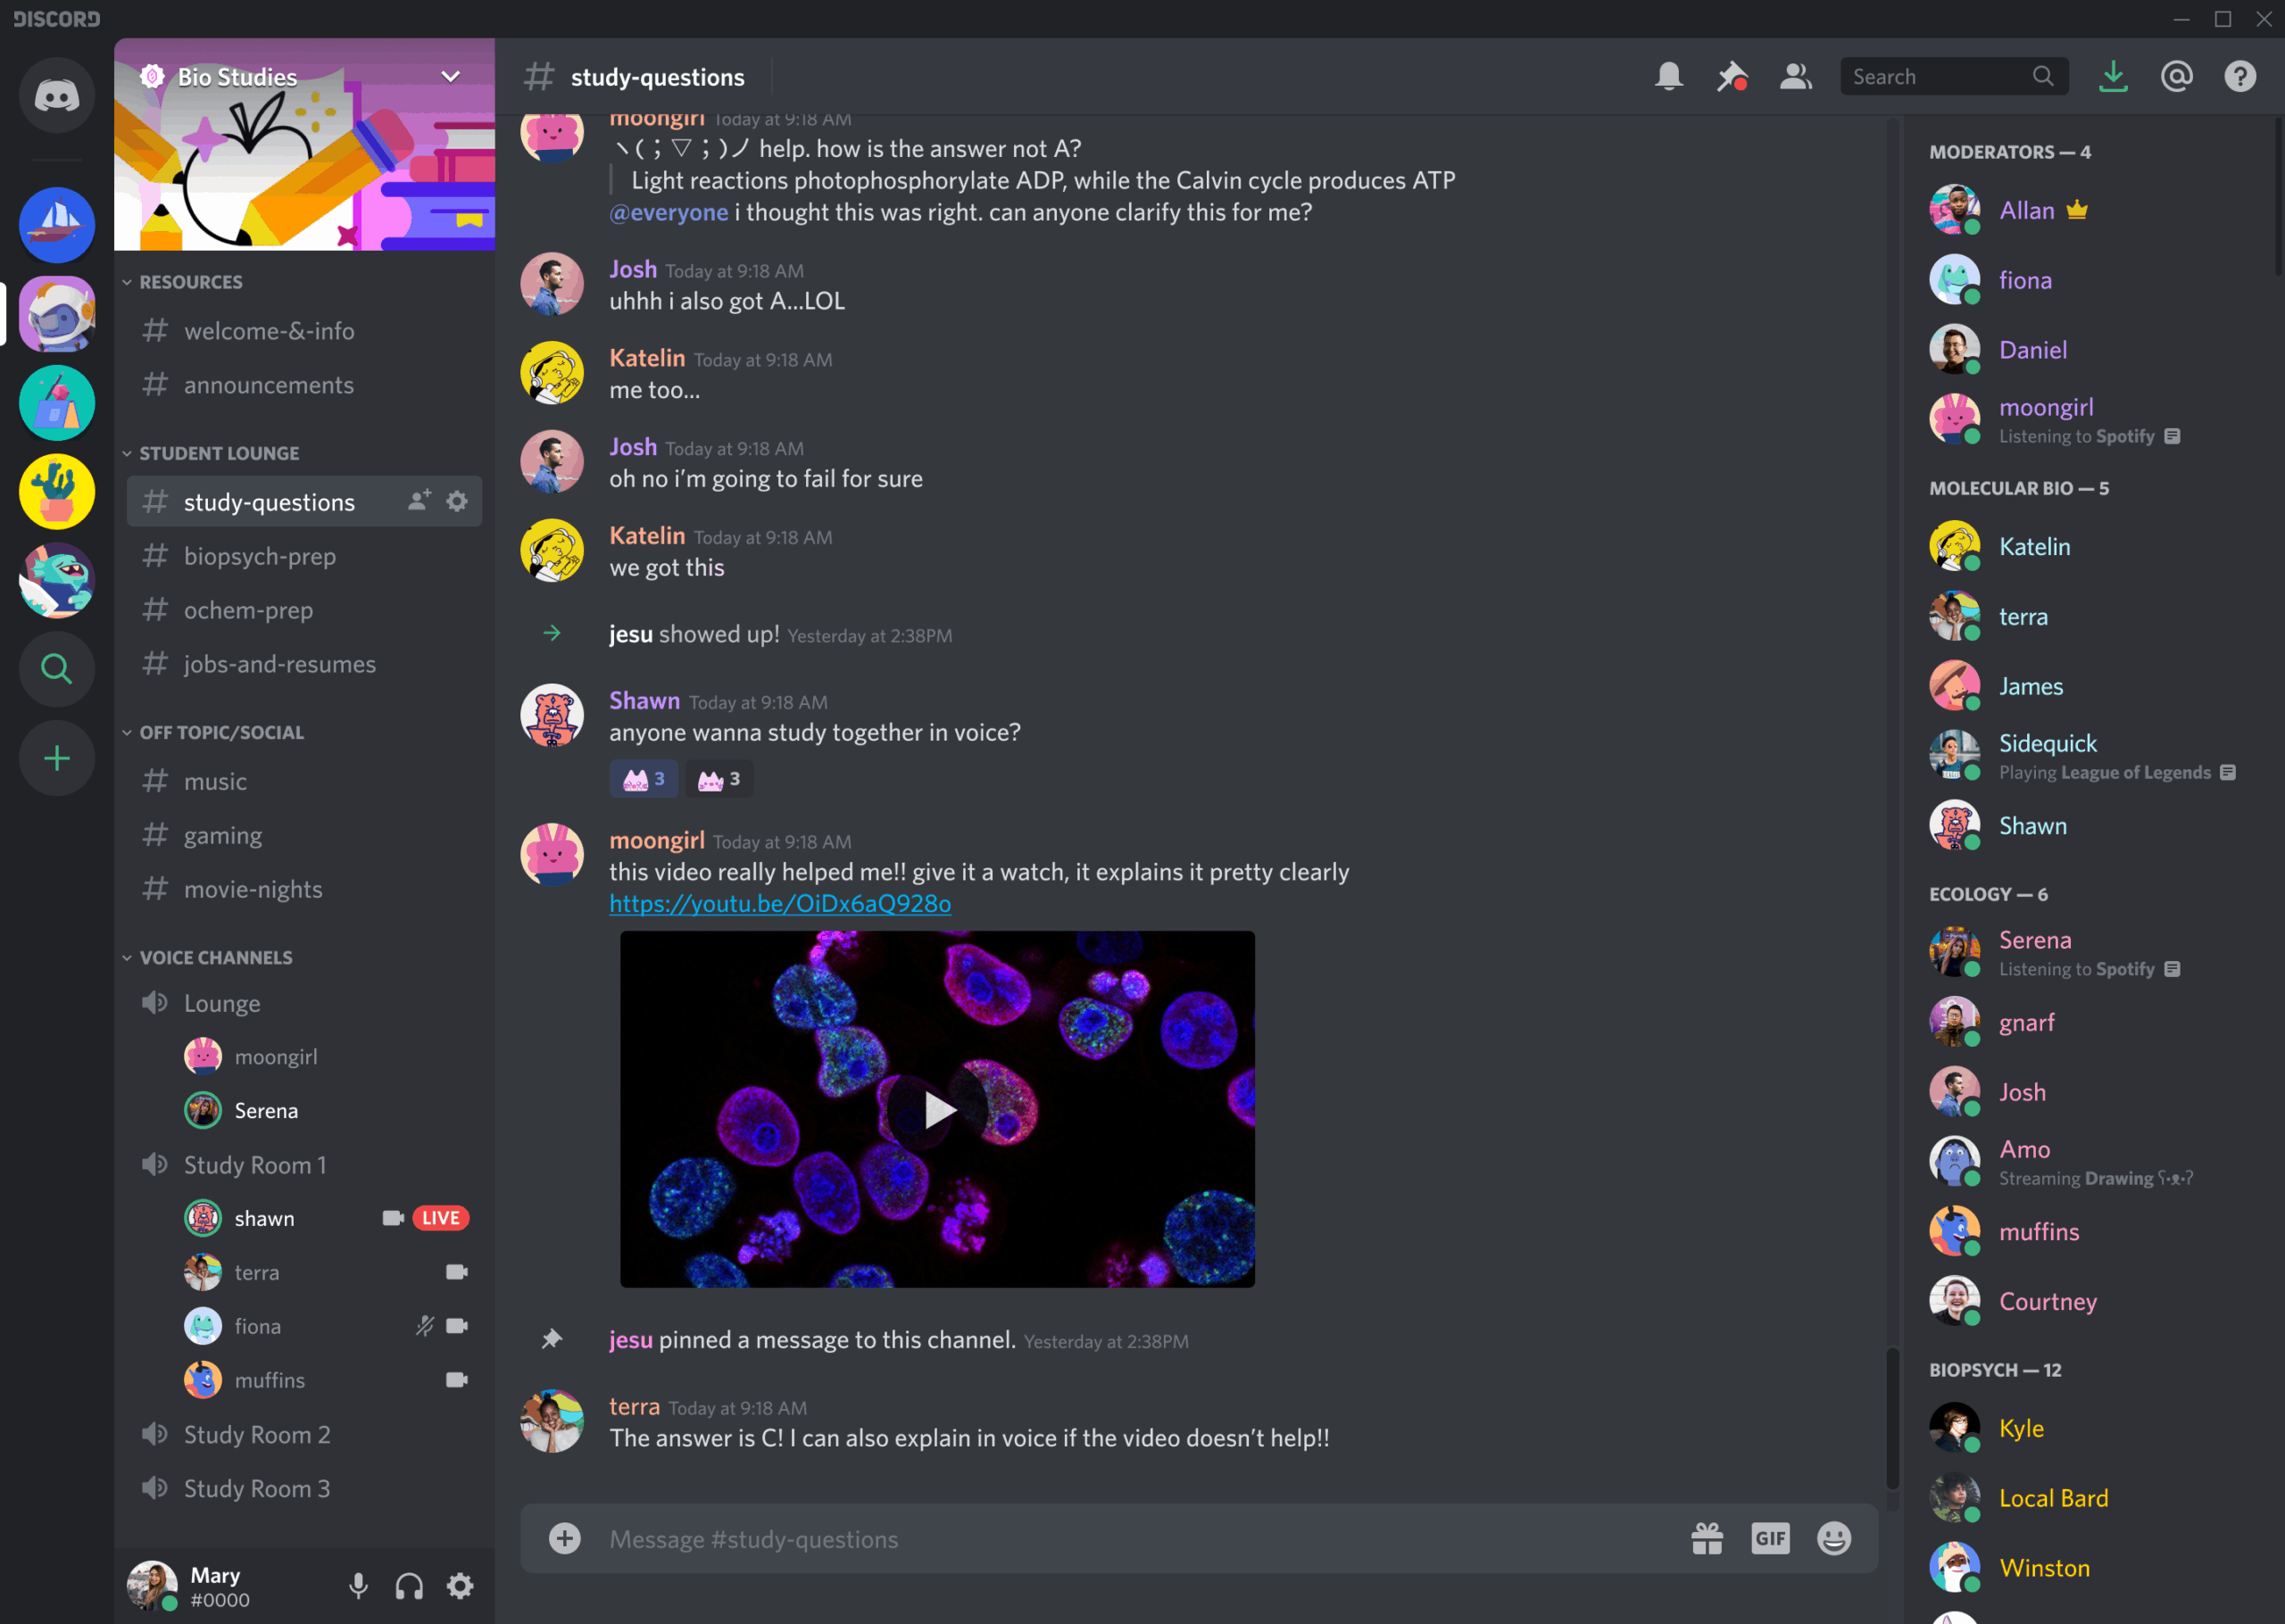
\includegraphics[width=1\textwidth]{img/discord.png}
	\caption{Interfaz web de \textit{Discord}.}
\end{figure}



\subsection{Bots}

Los bots son programas informáticos con funcionalidades definidas que pueden ser ejecutadas de forma autónoma o a voluntad de un usuario. Estos pueden ser de muchos tipos, como por ejemplo:

\begin{itemize}
	\item \textit{Chatbots}. Que intentan simular conversaciones humanas con el usuario.
	\item Maliciosos. Usados para difundir \textit{spam} o para realizar ataques informáticos.
	\item Sociales. Usados en aplicaciones sociales para realizar cualquier tipo de tarea.
\end{itemize}

En la estructura de un bot se pueden destacar dos partes principales. En primer lugar los comandos, que comprenderían la serie de órdenes concretas que el usuario puede indicar al bot que ejecute. Estos se describen en más amplitud en la siguiente sección. Por otro lado estarían una serie de módulos, que contienen el código fuente que ha creado el programador del bot, y que realizan las tareas deseadas tras la indicación del usuario mediante los comandos. Dichos módulos pueden tener multiples funciones, como el acceso a bases de datos, de inteligencia artificial, etc.

En concreto, los bots están compuestos por comandos y por distintos módulos. Los comandos son una serie de órdenes concretas que puede ejecutar el bot (más información en la siguiente sección). Por otro lado los módulos contienen el código fuente que ha creado un programador y que realizan las tareas deseadas. Los módulos pueden ser de acceso a bases de datos, de inteligencia artificial u otras características.

En cuanto al aspecto técnico, los bots se pueden crear con casi cualquier lenguaje de programación, haciendo uso de las distintas librerías y recursos disponibles. En el caso de los bots sociales, se utilizan librerías que actúan como capa de acceso a las \textit{API} que proveen las aplicaciones de este tipo.

Generalmente los bots operan a través de internet, siendo alojados en un servidor y se accede a sus funcionalidades mediante los mencionados comandos. Por tanto, cuando este software se ejecuta, queda a la escucha de los diferentes eventos que se lanzan por parte de los usuarios, preparado para ejecutar las tareas deseadas.

A continuación se muestra un ejemplo de bot de \textit{Discord} escrito en \textit{JavaScript}, de manera muy reducida:

\begin{lstlisting}
const client = new Client({ ... });

client.once('ready', () => {
    console.log('Ready!');
});

client.on('interactionCreate', async interaction => {
    if (!interaction.isCommand()) return;

    const { commandName } = interaction;
    
    if (!commandName.startsWith('!')) {
    	return;
    }

    if (commandName === 'ping') {
        await interaction.reply('Pong!');
    } else if (commandName === 'beep') {
        await interaction.reply('Boop!');
    }
});

client.login(token);
\end{lstlisting}


\subsection{Comandos}

Los comandos son órdenes o instrucciones concretas que, a petición del usuario, se ejecutan en cualquier momento. Se invocan haciendo uso de una palabra clave, aunque pueden ser también tareas fijas y programadas que se ejecuten de manera automática sin intervención de un usuario. Además, estos suelen admitir parámetros o argumentos, algo que permite modificar su comportamiento.

Para un usuario común estos comandos son simples mensajes que se escriben en un canal de texto, a los cuales reacciona el bot devolviendo una respuesta. En cambio, para el sistema subyacente, un comando es el gatillo que activa la ejecución de cierta tarea. Estas tareas pueden ser cualesquiera, siempre y cuando se puedan programar mediante código en el bot.

Un ejemplo sencillo puede ser enviar un mensaje de texto sencillo. Algo más complejo podría ser acceder a cierta \textit{API} meteorológica para consultar la previsión de la ciudad que el usuario incluye al ejecutar el comando.

Los comandos suelen ejecutarse precedidos de un \textit{token} o carácter clave, como \textit{!} o \textit{>}. La razón de ello es meramente la de distinguir los comandos de palabras usuales, además de para evitar confusiones al ejecutar los mismos. Esto no es un requisito indispensable, por lo que se puede omitir.

Por la parte del servidor que aloja al bot los comandos se suelen recibir como eventos, donde se incluye información como el contenido del mensaje enviado por el usuario, quién lo ha invocado, el canal donde se ha enviado el mensaje y otros parámetros que permiten identificar el contexto de ejecución.

A continuación se muestra la ejecución de los dos comandos configurados en el código de la sección anterior:

\begin{figure}[H]
	\centering
	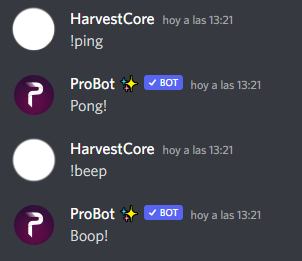
\includegraphics[width=0.5\textwidth]{img/commands.png}
	\caption{Ejemplo de ejecución de comandos en \textit{Discord}.}
\end{figure}



\section{Estructura del documento}

En este documento se explica el desarrollo del proyecto, llamado \textbf{Matroos}, por completo, desde decisiones que se han tomado hasta los distintos aspectos que se han tenido en cuenta.

Una vez introducido el problema, la motivación y algunos conceptos básicos se continúa por un repaso al estado del arte en el capítulo dos. Tras eso, en el capítulo tres, se desarrolla el análisis realizado al problema, indicando las personas implicadas, una serie de historias de usuario obtenidas y finalizando con el modelo de negocio que se podría aplicar para sacar rentabilidad al producto.

El capítulo cuatro introduce la planificación que se ha planteado para el desarrollo del proyecto, seguido del diseño técnico detallado en bastante profundidad en el capítulo cinco. Este incluye todas las pequeñas partes que componen la estructura y arquitectura interna del software creado.

Los dos siguientes capítulos, seis y siete, corresponden a las herramientas y tecnologías que se han utilizado y al desarrollo del software como tal, respectivamente. En el caso del segundo se incluyen detalles más técnicos, como código o archivos de configuración.

Finalmente, el capítulo ocho incluye las conclusiones que se han extraído tras el trabajo realizado en este proyecto, además de un listado de posibles áreas donde se podría mejorar el software en posteriores iteraciones.

De manera anexa se incluye la especificación de los \textit{endpoints} de los microservicios creados, así como un listado con las distintas variables de entorno usadas para configurar el software y una pequeña guía para ejecutar el mismo.

